%% Bookheader, Nov 8, 2020; July 18, 2022

\documentclass[11pt]{../Support/ourbook}
%% or for landscape, comment out line above and use this one:
%%\documentclass[landscape,11pt]{ourbook}

%% This will keep space from stretching around display math:

\makeatletter
\renewcommand\normalsize{%
   \@setfontsize\normalsize\@xipt{13.6}%
   \abovedisplayskip 11\p@  \@minus6\p@
   \abovedisplayshortskip \z@ 
   \belowdisplayshortskip 6.5\p@ \@minus3\p@
   \belowdisplayskip \abovedisplayskip
   \let\@listi\@listI}
\makeatother
\normalsize


\begin{document}

\tableofcontents
\graphicspath{{../../Chapters/differentiating_polynomials/en_US}}
\chapter{Differentiating Polynomials}

If you had a function that gave you the height of an object, it would
be handy to be able to figure out a function that gave you the
velocity at which it was rising or falling. The process of converting
the position function into a velocity function is known as
\emph{differentiation} or \emph{finding the derivative}.

There are a bunch of rules for finding a derivative, but
differentiating polynomials only requires three:
\begin{itemize}
\item The derivative of a sum is equal to the sum of the derivatives.
\item The derivative of a constant is zero.
\item The derivative of a nonconstant monomial $at^b$ ($a$ and $b$ are constant numbers, $t$ is time) is $abt^{b-1}$ 
\end{itemize}\index{differentiation!polynomials}

So, for example, if I tell you that the height in meters of quadcopter
at second $t$ is given by $2t^3 - 5t^2 + 9t + 200$. You could tell me
that its vertical velocity is $6t^{2} - 10t + 9$.

We indicate the derivative of a function with an apostrophe (read as "prime") between the name of the function and the variable. For example, the derivative of $h(t)$ is $h'(t)$ (which is read out loud as "h prime of t"). 

\begin{Exercise}[title={Differentiation of polynomials}, label=diffpoly]
  Differentiate the following polynomials.
  \begin{enumerate}
  \item $f(t)=2t^3-3t^2-4t$
  \item $g(t)=2t^{-3/4}$
  \item $F(r) = \frac{5}{r^3}$
  \item $H(u) = (3u-1)(u+2)$
  \end{enumerate}
  \end{Exercise}
\begin{Answer}[ref=diffpoly]
\begin{enumerate}
\item $f'(t) = 3t^2-6t-4$
\item $g'(t) = (\frac{-3}{4})2t^{-3/4-1}=\frac{-3}{2}t^{-7/4}$
\item $F'(r) = \frac{-15}{r^4}$
\item First, we expand the function by multiplying out the two binomials: $(3u-1)(u+2)=3u^2+6u-u-2$. Therefore, $H(u) = 3u^2+5u-2$, and we can differentiate using what we've learned about differentiating polynomials. $H'(u) = 6u+5$. In a later chapter, you will learn the Product rule, which will allow you to differentiate this function without multiplying out the binomials. 
\end{enumerate}
\end{Answer}
Notice that the degree of the derivative is one less than the degree
of the original polynomial. (Unless, of course, the degree of the
original is already zero.)

Now, if you know that a position is given by a polynomial, you can
differentiate it to find the object's velocity at any time.

The same trick works for acceleration: Let's say you know a function
that gives an object's velocity. To find its acceleration at any time,
you take the derivative of the velocity function (the second derivative). 

\begin{Exercise}[title={Differentiation of polynomials in Python}, label=pydiffpoly]
  Write a function that returns the derivative of a polynomial in \filename{poly.py}. It should look like this:
\begin{Verbatim}
def derivative_of_polynomial(pn):
  ...Your code here...
\end{Verbatim}
When you test it in \filename{test.py}, it should look like this:
\begin{Verbatim}
# 3x**3 + 2x + 5
p1 = [5.0, 2.0, 0.0, 3.0]
d1 = poly.derivative_of_polynomial(p1)
# d1 should be 9x**2 + 2
print("Derivative of", poly.polynomial_to_string(p1),"is", poly.polynomial_to_string(d1))

# Check constant polynomials
p2 = [-9.0]
d2 = poly.derivative_of_polynomial(p2)
# d2 should be 0.0
print("Derivative of", poly.polynomial_to_string(p2),"is", poly.polynomial_to_string(d2))
\end{Verbatim}
\end{Exercise}
\begin{Answer}[ref=pydiffpoly]
\begin{Verbatim}
def derivative_of_polynomial(pn):

    # What is the degree of the resulting polynomial?
    original_degree = len(pn) - 1
    if original_degree > 0:
        degree_of_derivative = original_degree - 1
    else:
        degree_of_derivative = 0

    # We can ignore the constant term (skip the first coefficient)
    current_degree = 1
    result = []

    # Differentiate each monomial
    while current_degree < len(pn):
        coefficient = pn[current_degree]
        result.append(coefficient * current_degree)
        current_degree = current_degree + 1

    # No terms? Make it the zero polynomial
    if len(result) == 0:
        result.append(0.0)

    return result
\end{Verbatim}
\end{Answer}

\section{Second order and higher derivatives}
As seen from the example with height, velocity, and acceleration, you can take the derivative of a derivative, which is called the second derivative and indicated with 2 marks, like so: 
$$\frac{d}{dx}f'(x) = f''(x)$$
When you have the height function (or position function, in the case of horizontal motion) of an object, the first derivative describes the velocity of the object, and the second derivative describes the acceleration. Suppose the motion of a particle is given by $s(t) = t^3-5t$, where $s$ is in meters and $t$ is in seconds.  What is the acceleration when the velocity is $0$? First, we find the velocity function, $s'(t)$, and the acceleration function, $s''(t)$:
$$s'(t) = 3t^2-5$$
$$s''(t) = 6t$$
To find where the velocity is $0$, set $s'(t) = 0$:
$$3t^2-5=0$$
$$3t^2=5$$
$$t^2=\frac{5}{3}$$
$$t = \sqrt{\frac{5}{3}} \approx 1.29s$$ (we ignore the other solution, $t=-\sqrt{\frac{5}{3}}$ because it is usual for time to start at zero.)

Next, we use $t\approx 1.29s$ in the acceleration function, $s''(t)$:
$$s''(\sqrt{\frac{5}{3}}) = 6\sqrt{\frac{5}{3}} \approx 7.75 \frac{m}{s^2}$$

For higher order derivatives, you just keep taking the derivative! So a third derivative is found by taking the derivative of the second derivative, and so on. 
\begin{Exercise}[title=Using Derivatives to Describe Motion, label=diffpoly2]
The position of a particle is described by the equation $s(t) = t^4-2t^3+t^2-t$, where $s$ is in meters and $t$ is in seconds. 

(a) Find the velocity and acceleration as functions of $t$.

(b) Find the velocity after 1.5 s. 

(c) Find the acceleration after 1.5 s.

(d) Is the object speeding up or slowing down at $t=1.5$? How do you know? 

\end{Exercise}
\begin{Answer}[ref=diffpoly2]
(a) Velocity is the first derivative of the position function, $s'(t) = 4t^3-6t^2+2t-1$. And acceleration is the derivative of the velocity function, $s''(t) = 12t^2-12t+2$. 

(b) $s'(1.5) = 4(1.5)^3-6(1.5)^2+2(1.5)-1 = 2$ We should note that this is a measurement and needs units to make sense. Since $s$ is in meters and $t$ is in seconds, our velocity should have units of $\frac{m}{s}$, so our final answer is $s'(1.5s) = 2\frac{m}{s}$. 

(c) $s''(1.5) = 12(1.5)^2-12(1.5)+2 = 11$. Similarly to part (b), our answer needs units. The units for acceleration are the units for velocity divided by the unit for time (because acceleration is a rate of change of velocity), and our final answer should be $s''(1.5s) = 11\frac{m}{s^2}$.

(d) When velocity and acceleration are occurring in the same direction (i.e. have the same sign), the speed (the absolute value of velocity) is increasing. Since $s'(1.5s)$ and $s''(1.5s)$ are both $>0$, the speed of the object is increasing. 
\end{Answer}
\graphicspath{{../../Chapters/classes/en_US}}
\chapter{Python Classes}

The built-in types, like strings have functions associated with
them. So, for example, if you needed a string converted to uppercase,
you would call it's \pyfunction{upper()} function:
-
\begin{Verbatim}
my_string = "houston, we have a problem!"
louder_string = my_string.upper()
\end{Verbatim}
This would set \pyvar{louder\_string} to "HOUSTON, WE HAVE A PROBLEM!"
When a function is associated with a datatype like this, it called a
\emph{method}. A datatype with methods is known as a \emph{class}. The
data of that type is known as \emph{instance} of that class. For
example, in the example, we would say ``\pyvar{my\_string} is an instance of
the class \pytype{str}. \pytype{str} has a method called \pyfunction{upper}''

The function \pyfunction{type} will tell you the type of any data:
\begin{Verbatim}
  print(type(my_string))
\end{Verbatim}
This will output
\begin{Verbatim}
<class 'str'>
\end{Verbatim}

A class can also define operators.  \pyfunction{+}, for example, is
redefined by \pytype{str} to concatenate strings together:
\begin{Verbatim}
long_string = "I saw " + "15 people"
\end{Verbatim}

\section{Making a Polynomial class}

You have created a bunch of useful python functions for dealing with
polynomials. Notice how each one has the word ``polynomial'' in the
function name like \pyfunction{derivative\_of\_polynomial}.  Wouldn't it
be more elegant if you had a Polynomial class with a
\pyfunction{derivative} method? Then you could use your polynomial
like this:\index{class in python}
\begin{Verbatim}
a = Polynomial([9.0, 0.0, 2.3])
b = Polynomial([-2.0, 4.5, 0.0, 2.1])

print(a, "plus", b , "is", a+b)
print(a, "times", b , "is", a*b)
print(a, "times", 3 , "is", a*3)
print(a, "minus", b , "is", a-b)

c = b.derivative()

print("Derivative of", b ,"is", c)
\end{Verbatim}

And it would output:
\begin{Verbatim}
2.30x^2 + 9.00 plus 2.10x^3 + 4.50x + -2.00 is 2.10x^3 + 2.30x^2 + 4.50x + 7.00
2.30x^2 + 9.00 times 2.10x^3 + 4.50x + -2.00 is 4.83x^5 + 29.25x^3 + -4.60x^2 + 40.50x + -18.00
2.30x^2 + 9.00 times 3 is 6.90x^2 + 27.00
2.30x^2 + 9.00 minus 2.10x^3 + 4.50x + -2.00 is -2.10x^3 + 2.30x^2 + -4.50x + 11.00
Derivative of 2.10x^3 + 4.50x + -2.00 is 6.30x^2 + 4.50  
\end{Verbatim}

Create a file for your class definition called \filename{Polynomial.py}. Enter the following:
\begin{Verbatim}
class Polynomial:
    def __init__(self, coeffs):
        self.coefficients = coeffs.copy()

    def __repr__(self):
        # Make a list of the monomial strings
        monomial_strings = []

        # For standard form we start at the largest degree
        degree = len(self.coefficients) - 1

        # Go through the list backwards
        while degree >= 0:
            coefficient = self.coefficients[degree]

            if coefficient != 0.0:
                # Describe the monomial
                if degree == 0:
                    monomial_string = "{:.2f}".format(coefficient)
                elif degree == 1:
                    monomial_string = "{:.2f}x".format(coefficient)
                else:
                    monomial_string = "{:.2f}x^{}".format(coefficient, degree)
                
                # Add it to the list
                monomial_strings.append(monomial_string)
        
            # Move to the previous term
            degree = degree - 1

        # Deal with the zero polynomial
        if len(monomial_strings) == 0:
            monomial_strings.append("0.0")
    
        # Separate the terms with a plus sign
        return " + ".join(monomial_strings)

    def __call__(self, x):
        sum = 0.0  
        for degree, coefficient in enumerate(self.coefficients):
            sum = sum + coefficient * x ** degree
        return sum

    def __add__(self, b):
        result_length = max(len(self.coefficients), len(b.coefficients))
        result = []
        for i in range(result_length):
            if i < len(self.coefficients):
                coefficient_a = self.coefficients[i]
            else:
                coefficient_a = 0.0

            if i < len(b.coefficients):
                coefficient_b = b.coefficients[i]
            else:
                coefficient_b = 0.0
            result.append(coefficient_a + coefficient_b)
            
        return Polynomial(result)

    def __mul__(self, other):

        # Not a polynomial?
        if not isinstance(other, Polynomial):
            # Try to make it a constant polynomial
            other = Polynomial([other])
        
        # What is the degree of the resulting polynomial?
        result_degree = (len(self.coefficients) - 1) + (len(other.coefficients) - 1)

        # Make a list of zeros to hold the coefficents
        result = [0.0] * (result_degree + 1)

        # Iterate over the indices and values of a
        for a_degree, a_coefficient in enumerate(self.coefficients):

            # Iterate over the indices and values of b
            for b_degree, b_coefficient in enumerate(other.coefficients):

                # Calculate the resulting monomial
                coefficient = a_coefficient * b_coefficient
                degree = a_degree + b_degree
            
                # Add it to the right bucket
                result[degree] = result[degree] + coefficient
            
        return Polynomial(result)

    __rmul__ = __mul__

    def __sub__(self, other):
        return self + other * -1.0
    
    def derivative(self):

        # What is the degree of the resulting polynomial?
        original_degree = len(self.coefficients) - 1
        if original_degree > 0:
            degree_of_derivative = original_degree - 1
        else:
            degree_of_derivative = 0

        # We can ignore the constant term (skip the first coefficient)
        current_degree = 1
        result = []

        # Differentiate each monomial
        while current_degree < len(self.coefficients):
            coefficient = self.coefficients[current_degree]
            result.append(coefficient * current_degree)
            current_degree = current_degree + 1

        # No terms? Make it the zero polynomial
        if len(result) == 0:
            result.append(0.0)

        return Polynomial(result)
\end{Verbatim}

Create a second file called \filename{test\_polynomial.py} to test it:
\begin{Verbatim}[commandchars=\\\{\}]
from Polynomial import Polynomial

a = Polynomial([9.0, 0.0, 2.3])
b = Polynomial([-2.0, 4.5, 0.0, 2.1])

print(a, "plus", b , "is", a+b)
print(a, "times", b , "is", a*b)
print(a, "times", 3 , "is", a*3)
print(a, "minus", b , "is", a-b)

c = b.derivative()

print("Derivative of", b ,"is", c)

slope = c(3)
print("Value of the derivative at 3 is", slope)

\end{Verbatim}

Run the test code:
\begin{Verbatim}
python3 test_polynomial.py
\end{Verbatim}

\graphicspath{{../../Chapters/common_products_polynomials/en_US}}
\chapter{Common Polynomial Products}

In math and physics, you will run into certain kinds of polynomials
over and over again. In this chapter, We are going to cover some
patterns that you will want to be able to recognize.

\section{Difference of squares}

Watch \textbf{Polynomial special products: difference of squares} from Khan Academy at \url{https://youtu.be/uNweU6I4Icw}.

If you are asked what $(3x - 7)(3x + 7)$ is, you would use the
distributive property to expand that to $(3x)(3x) + (3x)(7) + (-7)(3x) + (-7)(7)$.
Two of the terms cancel each other, so this is $(3x)^2 - (7)^2$. This would simplify to $9x^2 - 49$

You will see this pattern often. Anytime you see $(a + b)(a - b)$, you should immediately
recognize it equals $a^2 - b^2$. (Note that the order doesn't matter: $(a - b)(a + b)$ also $a^2 - b^2$.)

Working the other way is important too. Any time you see $a^2 - b^2$,
that you should recognize that you can change that into the product
$(a + b)(a - b)$. Making something into a product like this is known as
\emph{factoring}. You probably have done prime factorization of
numbers like $42 = 2 \times 3 \times 7$. In the next couple of
chapters, you will learn to factorize polynomials.

\begin{Exercise}[title={Difference of Squares}, label=diffsquares]
  Simplify the following products:
  \Question{$(2x - 3)(2x + 3)$}
  \Question{$(7 + 5x^3)(7 - 5x^3)$}
  \Question{$(x - a)(x + a)$}
  \Question{$(3 - \pi)(3 + \pi)$}
  \Question{$(-4x^3 + 10)(-4x^3 - 10)$}
  \Question{$(x + \sqrt{7})(x - \sqrt{7})$}
  Factor the following polynomials:
    \Question{$x^2 - 9$}
    \Question{$49 - 16x^6$}
    \Question{$\pi^2 - 25x^8$}
    \Question{$x^2 - 5$}
\end{Exercise}
\begin{Answer}[ref=diffsquares]
  $(2x - 3)(2x + 3) = 4x^2 - 9$
  
  $(7 + 5x^3)(7 - 5x^3) = 49 - 25x^6$
  
  $(x - a)(x + a) = x^2 - a^2$
  
  $(3 - \pi)(3 + \pi) = 9 - \pi^2$
  
  $(-4x^3 + 10)(-4x^3 - 10) = 16x^6 - 100$
  
  $(x + \sqrt{7})(x - \sqrt{7}) = x^2 - 7$

  $x^2 - 9 = (x + 3)(x - 3)$

  $49 - 16x^6 = (7 + 4x^3)(7 + 4^3)$
  
  $\pi^2 - 25x^8 = (\pi + 5x^4)(\pi - 5x^4)$
  
  $x^2 - 5 = (x + \sqrt{5})(x - \sqrt{5})$

\end{Answer}

We are often interested in the roots of a polynomial. That is, we want
to know ``For what values of $x$ does the polynomial evaluate to
zer?'' For example, when you deal with falling bodies, the first
question you might ask would be ``How many seconds before the hammer
hits the ground?''  Once you have factored a polynomial into
binomials, you can easily find the roots.

For example, what are the roots of $x^2 - 5$? You just factored it
into $(x + \sqrt{5})(x - \sqrt{5})$ This product is zero if and only
if one of the factors is zero. The first factor is only zero when $x$
is $-\sqrt{5}$. The second factor is zero only when $x$ is
$\sqrt{5}$. Those are the only two roots of this
polynomial.

Let's check that result. $\sqrt{5}$ is a little more than 2.2.  Using
your Python code, you can graph the polynomial:
\begin{Verbatim}
import poly.py
import matplotlib.pyplot as plt

# x**2 - 5
pn = [-5.0, 0.0, 1.0]

# These lists will hold our x and y values
x_list = []
y_list = []

# Start at x=-3
current_x =-3.0

# End at x=3.0
while current_x < 3.0:
    current_y = poly.evaluate_polynomial(pn, current_x)

    # Add x and y to respective lists
    x_list.append(current_x)
    y_list.append(current_y)

    # Move x forward
    current_x += 0.1

# Plot the curve
plt.plot(x_list, y_list)
plt.grid(True)
plt.show()
\end{Verbatim}

You should get a plot like this:

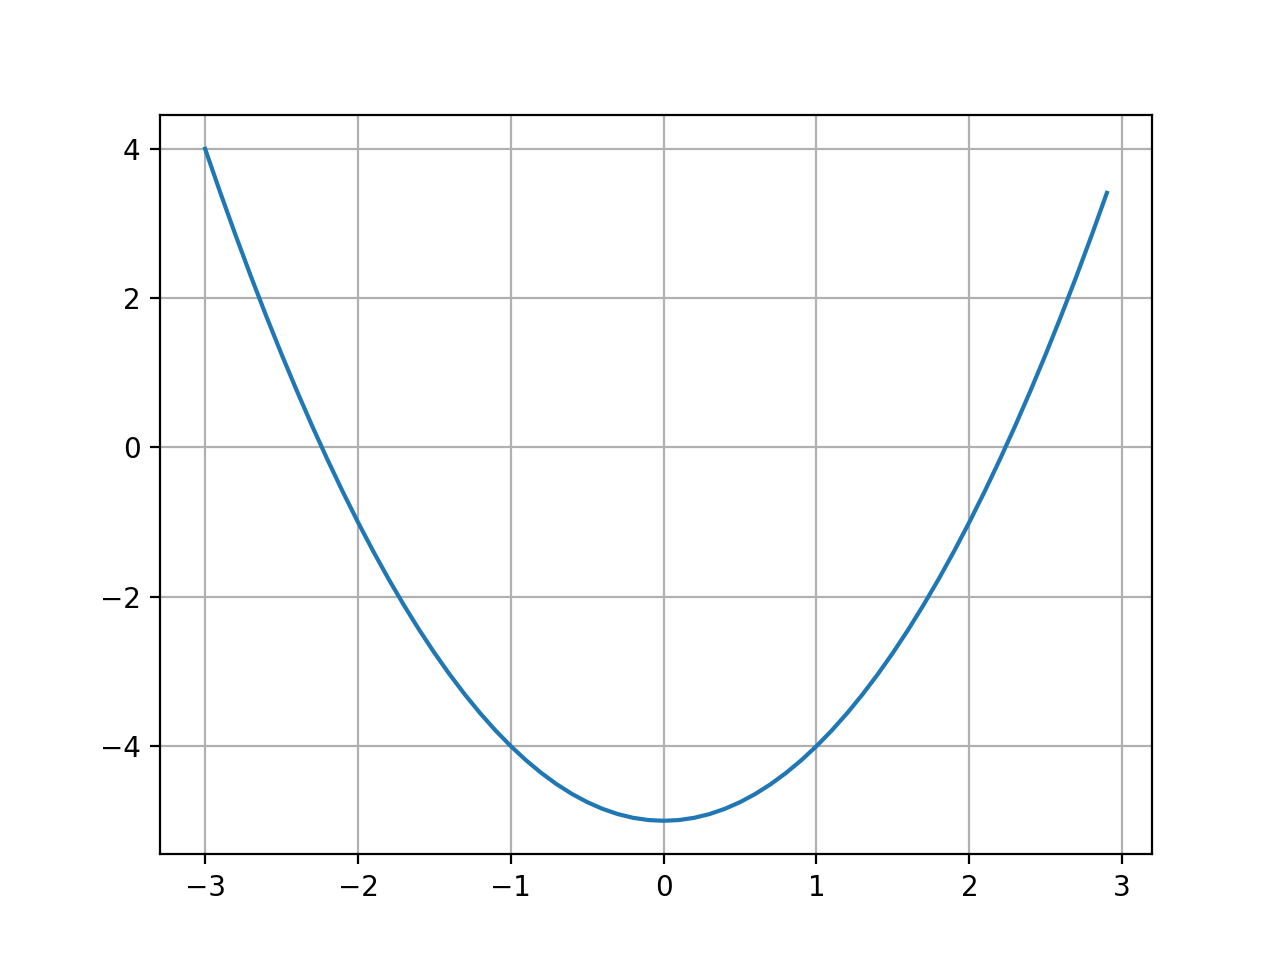
\includegraphics[width=\textwidth]{sqrt5.png}

It does, indeed, seem to cross the x-axis near -2.2 and 2.2.

\section{Powers of binomials}

You can raise whole polynomials to exponents. For example,
\begin{multline*}
  (3x^3 + 5)^2 = (3x^3 + 5)(3x^3 + 5) \\ = 9x^6 + 15x^3 + 15x^3 + 25 = 9x^6 + 30x^3 + 25 
\end{multline*}

A polynomial with two terms is called a \emph{binomial}. $5x^9 - 2x^4$,
for example, is a binomial. In this section, we are going to
develop some handy techniques for raising a binomial to some power.

Looking at the previous example, you can see that for any monomials $a$ and $b$, $(a + b)^2 = a^2 + 2ab + b^2$.
So, for example, $(7x^3 + \pi)^2 = 49x^6 + 14\pi x^3 + \pi^2$

\begin{Exercise}[title={Squaring binomials}, label=squaringbinomials]
  Simply the following
  \Question{$(x + 1)^2$}
  \Question{$(3x^5 + 5)^2$}
  \Question{$(x^3 - 1)^2$}
  \Question{$(x - \sqrt{7})^2$}
  
\end{Exercise}
\begin{Answer}[ref=squaringbinomials]
  $(x+1)^2 = x^2 + 2x + 1$

  $(3x^5 + 5)^2 = 9x^10 + 30x^5 + 25$

  $(x^3 - 1)^2 = x^6 - 2x^3 + 1$

  $(x - \sqrt{7})^2 = x^2 - 2x\sqrt{7} + 7$
\end{Answer}

What about $(x + 2)^3$? You can do it as two separate multiplications:
\begin{multline*}
  (x+2)^3 = (x+2)(x+2)(x+2) \\
  = (x + 2)(x^2 + 4x + 4) = x^3 + 4x^2 + 4x + 2x^2 + 8x + 8 \\
  = x^3 + 6x^2 + 12x + 8
\end{multline*}
In general, we can say that for any monomials $a$ and $b$, $(a + b)^3 = a^3 + 3a^2b + 3ab^2 + b^3$.

What about higher powers? $(a + b)^4$, for example? You could use the
distributive property four times, but it starts to get pretty tedious.

Here is a trick. This is known as \emph{Pascal's triangle}
\begin{equation*}
\begin{array}{c}
 1 \\
 1 \quad 1 \\
 1 \quad 2 \quad 1 \\
 1 \quad 3 \quad 3 \quad 1 \\
 1 \quad 4 \quad 6 \quad 4 \quad 1 \\
 1 \quad 5 \quad 10 \quad 10 \quad 5 \quad 1 \\
 1 \quad 6 \quad 15 \quad 20 \quad 15 \quad 6 \quad 1 \\
 1 \quad 7 \quad 21 \quad 35 \quad 35 \quad 21 \quad 7 \quad 1 \\
 \ldots
\end{array}
\end{equation*}
Each entry is the sum of the two above it.

The coefficients of each term are given by the entries in Pascal's triangle:
\begin{equation*}
(a + b)^4 = 1a^4 + 4a^3b + 6a^2 b^2 + 4 a b^3 + 1 b^4   
\end{equation*}

\begin{Exercise}[title={Using Pascal's Triangle}, label=pascalbinomial]
    \Question{What is $(x + \pi)^5$?}
\end{Exercise}
\begin{Answer}[ref=pascalbinomial]
  $(x + \pi)^5 = x^5 + 5\pi x^4 + 10\pi^2 x^3 + 10 \pi^3 + x^2 + 5 \pi^2 x + \pi^5$
\end{Answer}

\graphicspath{{../../Chapters/factoring_polynomials/en_US}}
\chapter{Factoring Polynomials}

We factor a polynomial into two or more polynomials of lower
degree. For example, let's say that you wanted to factor
$5x^3 - 45x$. You would note that you can factor out $5x$ from every term. Thus,
\begin{equation*}
5x^3 - 45x = (5x)(x^2 - 9)
\end{equation*}
You might notice that the second factor looks like the difference of squares, so
\begin{equation*}
5x^3 - 45x = (5x)(x + 3)(x - 3)
\end{equation*}
That is as far as we can factorize this polynomial.\index{factoring polynomials}

Why do we care? The factors make it easy to find the roots of the
polynomial. This polynomial evaluates to zero if and only if at least
one of the factors is zero. Here, we see that
\begin{itemize}
\item The factor $(5x)$ is zero when $x$ is zero.
\item The factor $(x + 3)$ is zero when $x$ is -3.
\item The factor$(x - 3)$ is zero when $x$ is 3.
\end{itemize}
So, looking at the factorization, you can see
that $5x^3 - 45x$ is zero when $x$ is 0, -3, or 3. 

This is a graph of that polynomial with its roots circled:

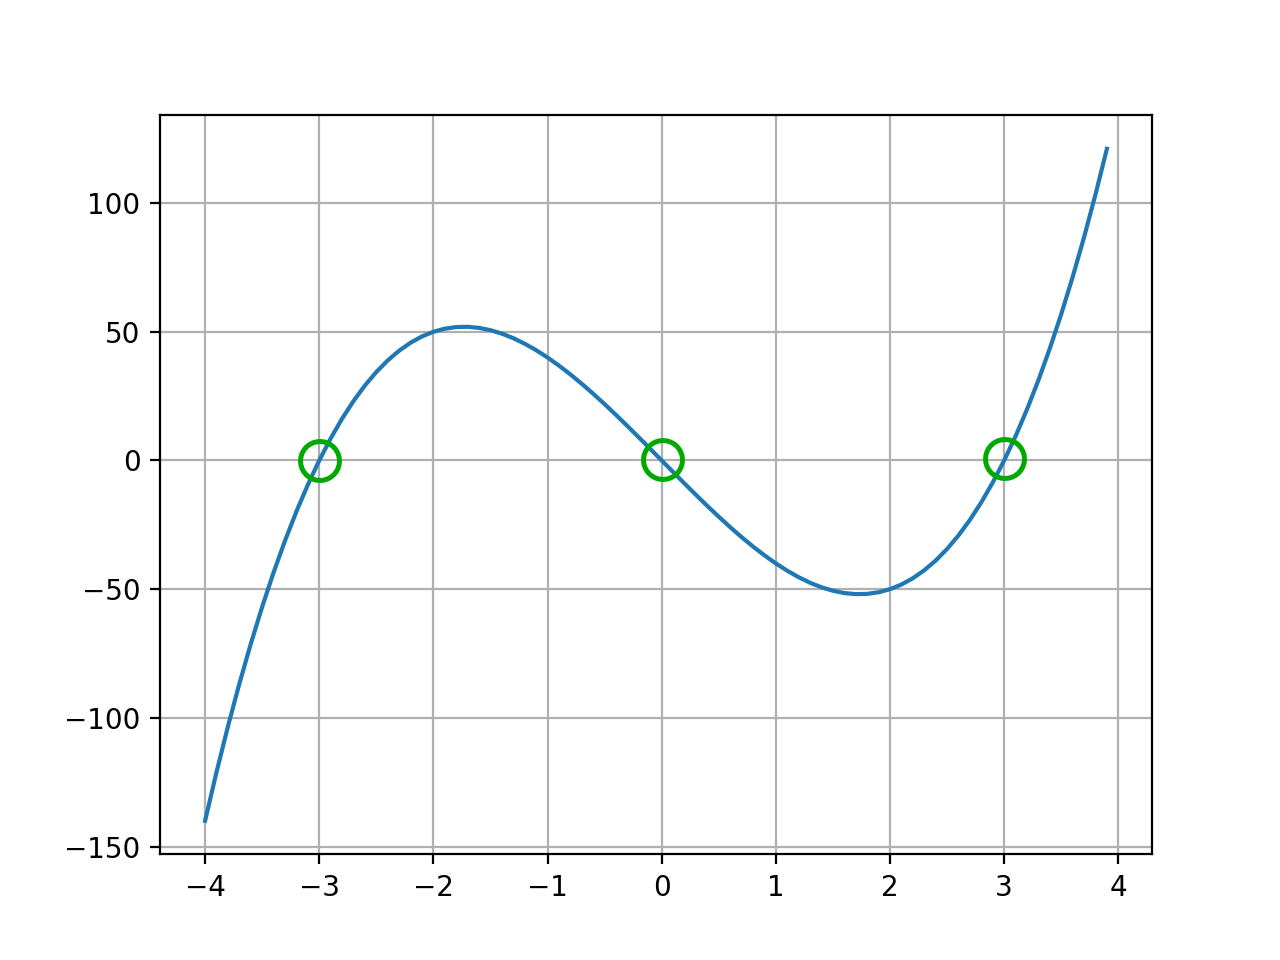
\includegraphics{factor4roots.png}

\section{How to factor polynomials}

The first step when you are trying to factor a polynomial is to find
the greatest common divisor for all the terms, then pull that out. In
this case, the greatest common divisor will also be a monomial. Its
degree is the least of the degrees of the terms, its coefficient will
be the greatest common divisor of the coefficients of the terms.

For example, what can you pull out of this polynomial?
\begin{equation*}
12x^100 + 30x^31 + 42x^17
\end{equation*}
The greatest common divisor of the coefficients (12, 30, and 42) is 6.  The least of the degrees of terms (100, 31, and 17) is 17.  So, you can pull out $6x^17$:
\begin{equation*}
12x^100 + 30x^31 + 42x^17 = (6x^17)(2x^83 + 5x^14 + 7)
\end{equation*}

\begin{Exercise}[title={Factoring out the GCD monomial}, label=gcdmonomial]
  
\end{Exercise}
\begin{Answer}[ref=gcdmonomial]
  
\end{Answer}

So, now you have the product of a monomial and a polynomial. If you
are lucky, the polynomial part looks familiar, like the difference of
squares or a row from Pascal's triangle.

Often, you are trying factor a quadratic like $x^2 + 5x + 6$ in a pair
of binomials. In this case, the result would be $(x + 3)(x + 2)$. Let's check that:
\begin{equation*}
  (x + 3)(x + 2) = (x)(x) + (3)(x) + (2)(x) + (3)(2) = x^2 + 5x + 6
\end{equation*}
Notice that 3 and 2 multiply to 6 and add to 5. If you were trying to
factor $x^2 + 5x + 6$, you would ask yourself''What are two numbers that
when multiplied equal 6 and when added equal 5?'' And you might
guess wrong a couple of times. For example, you might say to youself,
``Well, 6 times 1 is 6. Maybe those work. But 6 and 1 add 7. So those
don't work.''

Solving these sorts of problems are like solving a Sudoku puzzle. You
try things and realize they are wrong, so you backtrack and try
something else.

The numbers are sometimes negative. For example, $x^2 + 3x - 10$ factors into $(x + 5)(x - 2)$.

\begin{Exercise}[title={Factoring quadratics}, label=factorquadratics]
  
\end{Exercise}
\begin{Answer}[ref=factorquadratics]
  
\end{Answer}

%%%%%%%%%%%%%%%%%%%%%%%%%%%%%%%%%
%% Bookfooter.tex by Aaron Hillegass
%% Nov 8, 2020

\appendix

\chapter{Answers to Exercises}
\shipoutAnswer

\bibliography{references}

\printindex

\end{document}